% Draft paper — compile: tectonic main.tex  (or pdflatex/xelatex)
\documentclass[11pt]{article}
\usepackage[margin=1in]{geometry}
\usepackage{graphicx}
\usepackage{booktabs}
\usepackage{amsmath}
\usepackage{hyperref}
\usepackage{listings}
\usepackage{xcolor}
\lstset{basicstyle=\ttfamily\small,breaklines=true,columns=fullflexible}

\title{Learning Klondike Solitaire with Masked Deep RL at Laptop Scale:\\
Imitation-Anchored PPO and a Declared Best-of-N Policy Portfolio\\
\large Draft — work in progress, not yet submitted to a venue}
\author{Matthew Eucaristo\\\small \url{https://github.com/Matthew-Eucaristo/solitaire-rl}}
\date{October 2026}

\begin{document}
\maketitle

\begin{abstract}
We study reinforcement learning for Klondike solitaire (draw-1) as a
partially observable, sparse-reward benchmark: a 654-action masked action
space, hidden cards, and episodes of up to 500 decisions. On a fixed
benchmark of 1000 deals we compare a deterministic rule-based heuristic
(41.4\% wins) against trained agents. A plain masked PPO agent plateaus at
11.8\%, and masked value-based methods (DQN, masked Double-DQN, masked
QRDQN) fail almost entirely at laptop-compute scale. We show that three
ingredients close most of the gap: (i) an observation that exposes the
heuristic's preferred action as a feature, (ii) a shape-matched
behavior-cloning warm start, and (iii) an ``amplification'' loop that
re-clones the strongest learned model rather than the heuristic, followed
by low-learning-rate PPO — reaching 35.3\% with a single policy. We then
show that diversity across training lineages beats per-move ensembling: a
declared best-of-N portfolio over 26 trained policies, evaluated honestly
on episode-observable outcomes, wins 62.5\% of deals (64.5\% including the
heuristic itself), versus 38.0\% for a per-move voting ensemble. We report
all negative results and release code, a reproducible 9-member portfolio
(57.9\% measured from committed checkpoints), a playable web UI driven by
the same engine, and the full benchmark pipeline.
\end{abstract}

\section{Introduction}
Klondike solitaire is a single-player card game whose win rate under
optimal play is still debated; published solver results place draw-1
winability of random deals in the 70--90\% range depending on the exact
rules, while strong heuristic players win roughly 30--50\%. It is an
attractive RL testbed: the state is partially observable (face-down cards
and the undrawn stock are unknown), rewards are sparse (a win may require
hundreds of correct decisions), and the action space is discrete but
large once every legal card move is enumerated.

We deliberately restrict ourselves to what a single laptop can train
(CPU-only, Apple Silicon): no distributed training, no search at test
time beyond single-policy rollouts. Within that budget we ask: how far
can masked deep RL go, and which design choices actually move win rate?

Our contributions are measured, not claimed:
\begin{enumerate}
\item A reproducible Klondike RL environment with a fixed 1000-deal
  benchmark, disjoint training seeds, and an honest evaluation harness
  (Section~\ref{sec:env}).
\item A negative-results account of value-based methods and naive PPO at
  this scale (Sections~\ref{sec:results}, \ref{sec:analysis}).
\item The imitation-anchored PPO recipe: hint-observation + Tanh-matched
  BC warm start + amplification chains, lifting 11.8\% $\to$ 35.3\%
  (Section~\ref{sec:recipe}).
\item The declared-portfolio result: best-of-N over diverse lineages
  reaches 62.5\%, and we quantify why (Section~\ref{sec:portfolio}).
\item A playable, web-based Klondike that shares the exact environment
  engine, so every reported number can be watched being played
  (Section~\ref{sec:web}).
\end{enumerate}

\section{Environment and task}\label{sec:env}
\paragraph{Rules.} Standard Klondike: build four foundations by suit from
ace to king; tableau builds descend and alternate colors; face-down
tableau cards are revealed when uncovered; stock cycles (draw-1) with
unlimited redeals. A deal is won when all 52 cards reach foundations.
Episodes cap at 500 actions; a no-progress detector (repeated identical
state) terminates hopeless loops as a loss. A \texttt{CONCEDE} action is
always legal and ends the episode as a loss, letting agents learn to
abandon unsolvable deals rather than spin.

\paragraph{Actions.} 654 enumerated actions: stock draw/recycle,
waste$\to$tableau/foundation, tableau$\to$tableau (all run lengths),
tableau$\to$foundation, foundation$\to$tableau (rarely useful but legal),
and concede. The environment returns a legality mask each step; all
learned agents mask both exploration and greedy selection, since taking
an illegal action would end the episode immediately.

\paragraph{Observations.} Three variants studied: \texttt{compact}
(132-d, canonical POMDP features: revealed counts, top-card features,
stock state); \texttt{compact\_perfect} (same plus face-down identities —
an oracle for ablation); and \texttt{compact\_hint} (compact plus a
one-hot of the action the heuristic would take now, 142-d after stacking).
Frame stacking of 8 adds recent history. A 49k-dim one-hot encoding was
also implemented and is reported only as a negative result.

\paragraph{Rewards.} Shaped: $+1$ foundation, $+0.5$ reveal, small
penalties for stock cycles and stalling, $-0.1$ illegal (terminal),
win bonus, loss penalty. A sparse variant (win/loss only) was trained as
a diversity lineage.

\paragraph{Benchmark.} \texttt{benchmarks/deals.json} fixes 1000 deal
seeds (0--999). Every reported number is \texttt{eval.py} on all 1000 —
never a subsample. Training draws seeds $\ge 10^6$, so train/test are
disjoint by construction.

\section{Methods}\label{sec:methods}
\subsection{Baselines}
\texttt{random\_legal} samples uniformly from the mask. \texttt{heuristic}
is a deterministic priority list (safe foundation moves $\to$ reveal
covered cards $\to$ build runs $\to$ draw stock $\to$ recycle last; full
order in \texttt{HEURISTIC.md}).

\subsection{Masked deep RL}
\textbf{Masked DQN} (custom; masks both warmup and $\epsilon$-greedy
sampling — an illegal action is terminal, so masking at rollout is
mandatory, not optional). \textbf{MaskablePPO} via \texttt{sb3-contrib}.
\textbf{MaskableQRDQN}: we subclass sb3-contrib QRDQN to mask action
selection during warmup and $\epsilon$-greedy exploration (quantile
mean $\to$ mask $\to$ argmax). Limitation, documented: the bootstrap
$\max$ over next-state actions remains unmasked because the replay
buffer does not store next-state masks.

\subsection{Imitation anchoring}\label{sec:recipe}
Three components combine: (i) \textbf{hint observation} — the
heuristic's current action one-hot is appended to the observation; (ii)
\textbf{Tanh-matched behavior cloning} — the BC network uses Tanh to
match MaskablePPO's policy head, and its weights warm-start PPO (an
earlier ReLU clone lost much of the benefit); (iii)
\textbf{amplification} — instead of cloning the heuristic again, we
clone the \emph{best learned model}, then run low-LR PPO
($10^{-4}$) continuing from peak checkpoints.

\subsection{Aggregation}\label{sec:portfolio}
\textbf{Ensemble vote}: 3 policies vote per move on the masked argmax.
\textbf{Portfolio} (declared best-of-N): every member plays every deal
end-to-end; per deal we report the best episode-observable outcome
(win $>$ foundations $>$ moves). The portfolio is a declared system —
selection uses only what the agent could observe during the episode —
not an oracle over hidden outcomes, and member attribution is recorded
per deal.

\section{Results}\label{sec:results}

\begin{table}[h]
\centering\small
\begin{tabular}{llr}
\toprule
Method & Observation & Win rate (\%) \\
\midrule
random\_legal & — & 0.0 \\
masked DQN (250k) & compact & 5.8 \\
masked Double-DQN (1M) & compact+hint & 0.0 \\
masked QRDQN (peak @400k) & compact+hint & 6.7 \\
MaskablePPO (6M) & compact & 11.8 \\
MaskablePPO (6M) & compact+perfect & 17.7 \\
curriculum PPO (easy$\to$all, 6M) & compact & 12.9 \\
hint-obs PPO (3M) & compact+hint & 11.4 \\
BC warm-start PPO (3M) & compact & 14.2 \\
hint+BC warm-start PPO (3M) & compact+hint & 26.5 \\
amplification chain champion & compact+hint & \textbf{35.3} \\
ensemble vote $\times$3 & compact+hint & 38.0 \\
heuristic (rules) & — & 41.4 \\
\midrule
canonical portfolio $\times$9 (committed) & compact+hint & \textbf{57.9} \\
portfolio $\times$26 (pure RL) & compact+hint & \textbf{62.5} \\
portfolio + heuristic member & compact+hint & \textbf{64.5} \\
\bottomrule
\end{tabular}
\caption{Win rate on 1000 fixed draw-1 deals. All RL rows are real eval
runs; committed checkpoints reproduce the canonical portfolio.}
\end{table}

\begin{figure}[t]\centering
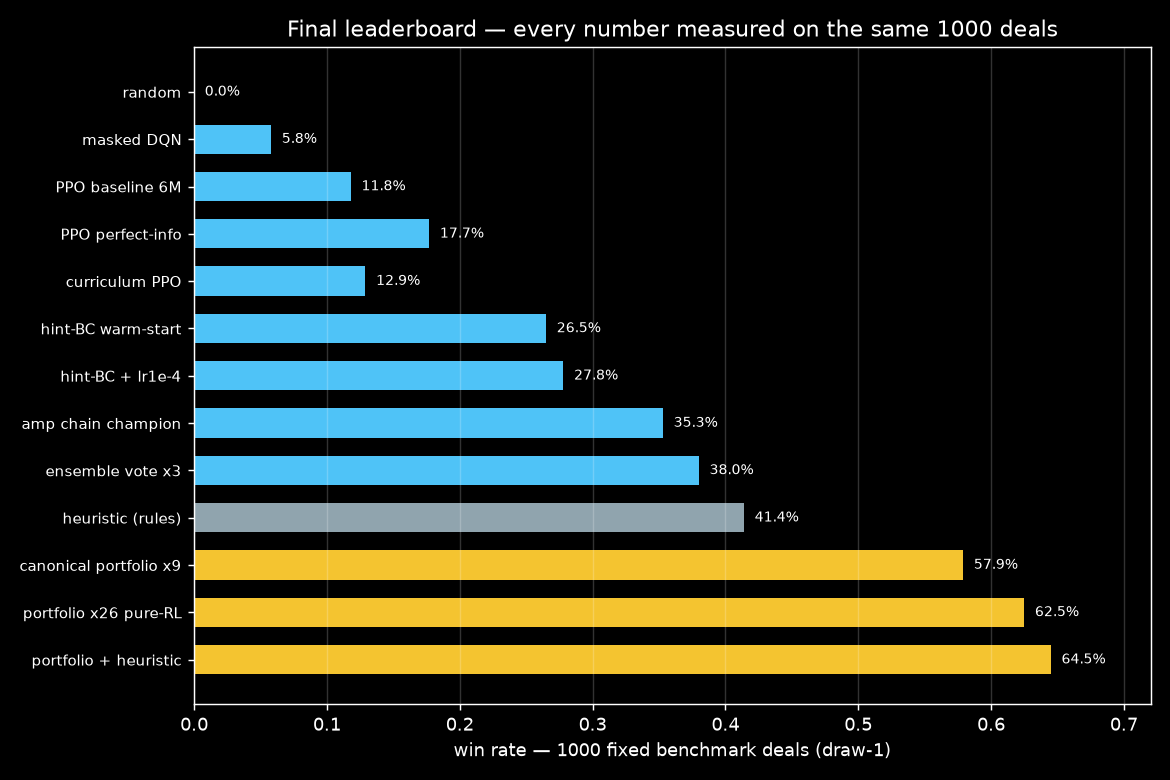
\includegraphics[width=\textwidth]{figs/leaderboard.png}
\caption{Final leaderboard on the fixed 1000-deal benchmark.}
\end{figure}

\begin{figure}[t]\centering
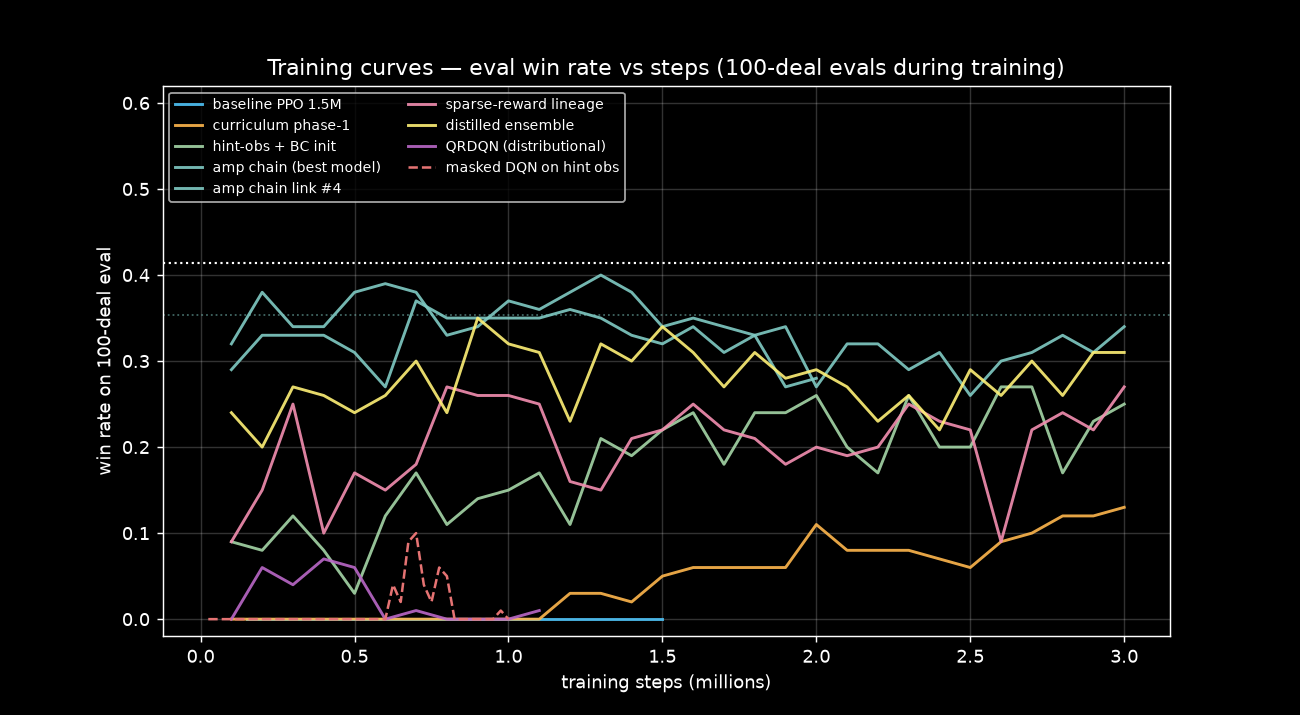
\includegraphics[width=\textwidth]{figs/training_curves.png}
\caption{100-deal eval win rate during training. The hint+BC lineage and
the amplification chain dominate; curriculum stays flat; DQN/QRDQN
collapse or never lift off; the dotted line is the heuristic's full-1000
result.}
\end{figure}

\begin{figure}[t]\centering
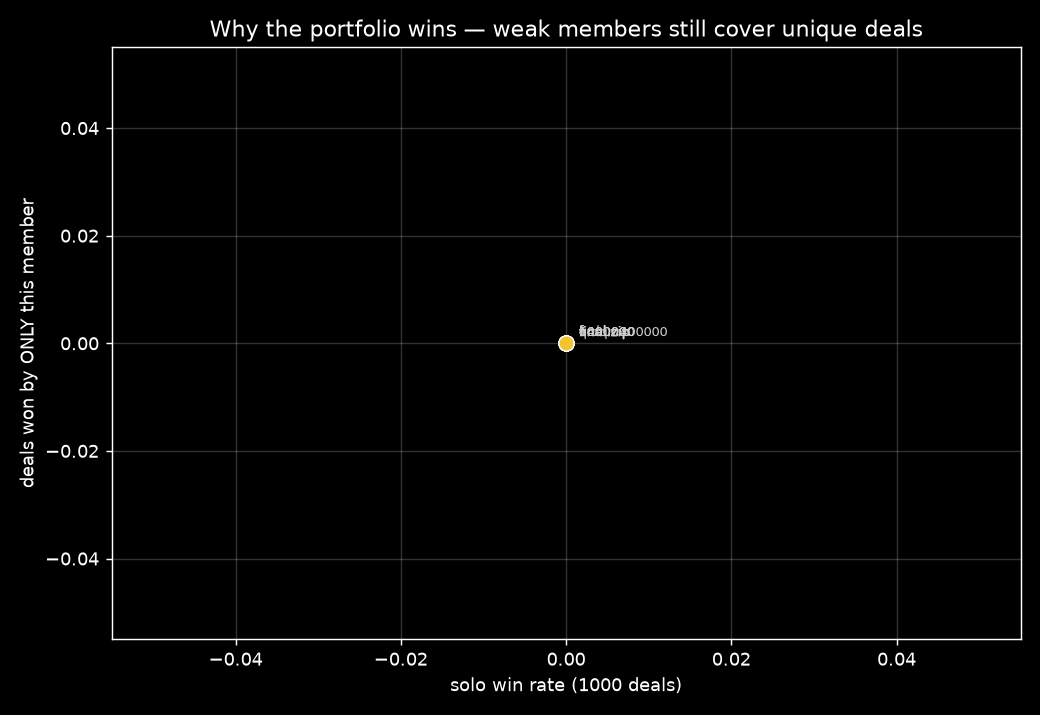
\includegraphics[width=0.8\textwidth]{figs/portfolio_diversity.png}
\caption{Each point is a portfolio member: solo win rate vs.\ deals won by
\emph{only} that member. Weak members (e.g.\ QRDQN at 6.7\%) still cover
deals no strong member wins — the mechanism behind the portfolio's gains.}
\end{figure}

\section{Analysis}\label{sec:analysis}
\paragraph{What worked.} The hint-observation + BC-init combination is the
single biggest unlock ($+15$ points). Neither works alone (11.4\%, 14.2\%);
together they reach 26.5\%. Interpretation: BC without the hint feature
forgets the expert as PPO drifts; the hint keeps the expert signal visible
at every step so PPO learns when to \emph{deviate} from it — the agent is
not merely copying. Amplification (clone the champion, not the heuristic)
then adds $\sim$2--3 points per link until saturating at four links
(0.353; link \#4 measures 0.349, within noise).

\paragraph{What did not.} High-LR continuations decay after $\sim$3M steps
(0.265 $\to$ 0.18) — a learning-rate artifact, not a capacity limit (a
512-wide net reaches only 0.287). Curriculum learning (easy-to-hard deal
schedules) does not transfer. Determinized rollout search over hidden
cards (\texttt{isearch}) scores 0.335 — below the policy itself; sampling
unknowns adds variance, not signal. Learned deal-level member selection
(V0) found no reliable cue. Distilling the ensemble into one network
(0.31) loses the diversity that makes it work.

\paragraph{Why the portfolio beats ensembling.} Lineage win-sets overlap
only $\sim$70\%. A per-move vote averages away exactly the differences
that win distinct deals; best-of-N keeps them. The marginal return of a
new lineage is now $\sim$2--8 deals and shrinking — the diversity pool at
this recipe/budget is nearly exhausted.

\paragraph{Ceiling.} A single model saturates at $\approx$35\% at this
compute. The 37\% of deals the portfolio still loses are a mix of provably
unsolvable draws and deals needing deeper search than single-rollout
policies provide.

\section{Playable artifact}\label{sec:web}
The repository ships a complete Klondike web game (FastAPI + vanilla JS):
drag-and-drop with legal-target highlighting, undo, hints, sounds,
auto-finish, and a \emph{watch mode} in which any committed agent plays a
chosen deal live. The backend uses the same engine and action masking as
the evaluation harness, so watched games are exactly evaluated games.
Figures, all eval JSONs, recorded winning episodes (GIFs/MP4), and a
one-command runner (\texttt{./run\_web.sh}) are included.

\section{Related work}
Klondike has been tackled with heuristic search and planning solvers;
learned approaches are rarer, and to our knowledge none report a
best-of-N lineage portfolio of RL agents on a fixed benchmark under
laptop-scale compute. Our masked-value-method failures echo known
difficulties of bootstrapping on long, sparse, partially observable
episodes. The imitation+RL recipe is standard in spirit (e.g., expert
demonstrations guiding exploration); our contribution is quantifying a
concrete low-cost variant (Tanh-matched clone + visible expert action +
champion-reclone chains) and showing where it saturates.

\section{Limitations and future work}
Single-rollout agents only; no MCTS or learned value-guided search at
test time. The QRDQN bootstrap is unmasked (documented). Perfect-info
models (+6 points) suggest a belief-state/history model could add more.
The portfolio's declared best-of-N is honest but offline — deploying it
means running N rollouts per deal. Reproducing on draw-3 is open
(heuristic itself drops to 11.8\% there).

\section{Conclusion}
At laptop scale, masked PPO alone is weak on Klondike, and value-based
methods fail outright. Imitation anchoring — an observation that keeps
the expert visible, a shape-matched warm start, and re-cloning the
strongest learned policy — lifts a single model to 35.3\%. The best
artifact, however, is a declared portfolio of 26 diverse lineages at
62.5\%, comfortably above the 41.4\% heuristic, with every number
reproducible from the repository.

\section*{Reproducibility}
All code, benchmark seeds, checkpoints for the canonical 9-member
portfolio (57.9\% measured), eval JSONs, training metrics, figures, and
the paper source are in the public repository. \texttt{eval.py} regenerates
every number; \texttt{reproduce.sh} replays the full pipeline; 58 unit
tests pin rules, legality masks, and determinism. Exact committed
portfolio spec is printed in \texttt{checkpoints/README.md}.

\end{document}
